% This text is proprietary.
% It's a part of presentation made by myself.
% It may not used commercial.
% The noncommercial use such as private and study is free
% Sep. 2005 
% Author: Sascha Frank 
% University Freiburg 
% www.informatik.uni-freiburg.de/~frank/


\documentclass[xcolor=table]{beamer}
\usepackage{beamerthemeshadow}
\usepackage{helvet}
\usepackage[]{graphicx}
\usepackage{array}
\begin{document}
\title{Python for Scientific Research}   
\author{Bram Kuijper} 
\date{\today} 

\frame{\titlepage} 


\frame{
    \frametitle{Course Schedule} 
    \begin{itemize}
        \item Today, March 6: The basics of programming in Python
            \begin{itemize}
                \item how to run Python code
                \item data types
                \item variable scope
                \item flow control
                \item text manipulation
            \end{itemize}
            \pause
        \item March 20th: Applying Python to simplify your life
            \begin{itemize}
                \item functions
                \item working with files
                \item working with data using \texttt{pandas} and \texttt{scipy}
                \item making graphs using \texttt{matplotlib}
            \end{itemize}
            \pause
        \item March 27th: Advanced subjects
            \begin{itemize}
                \item object-oriented programming
                \item automating tasks in MS-office
                \item image manipulation
                \item working on student-generated problems
            \end{itemize}
    \end{itemize}
}

\frame{
    \frametitle{Today's schedule} 
    \begin{itemize}
        \item 1300 - 1400: How to run Python \& Data types
        \item 1400 - 1420: Break
        \item 1420 - 1520: Variable scope \& Flow control
        \item 1520 - 1540: Break
        \item 1540 - 1640: Functions, working with files 
    \end{itemize}
}

\frame{\frametitle{What is Python?}
\begin{itemize}
    \item A scripted, high-level programming language created by Guido Van Rossum and named after Monty Python's flying circus
\begin{center}
    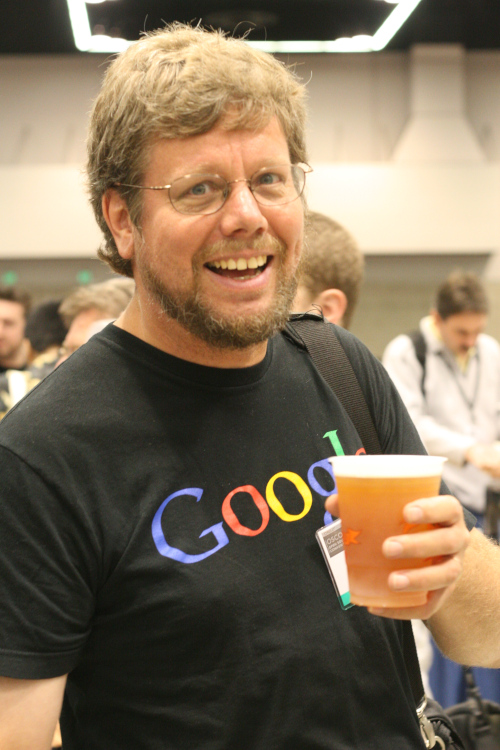
\includegraphics[width = 20mm]{img/GuidoVanRossumSmall.jpg}
    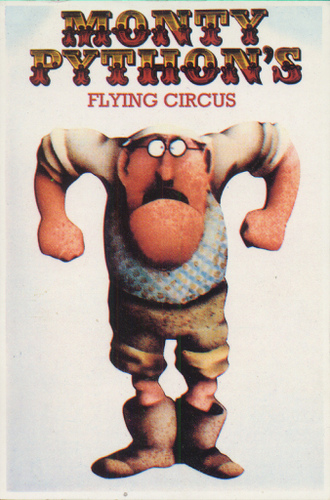
\includegraphics[width = 20mm]{img/MontyPython.jpg}
\end{center}
    \pause
    \item easy-to-use, highly standardized and with an emphasis on readability of code
\end{itemize}
}


\frame{\frametitle{Why use Python?}
The TIOBE index is a measure of the popularity of programming languages:
    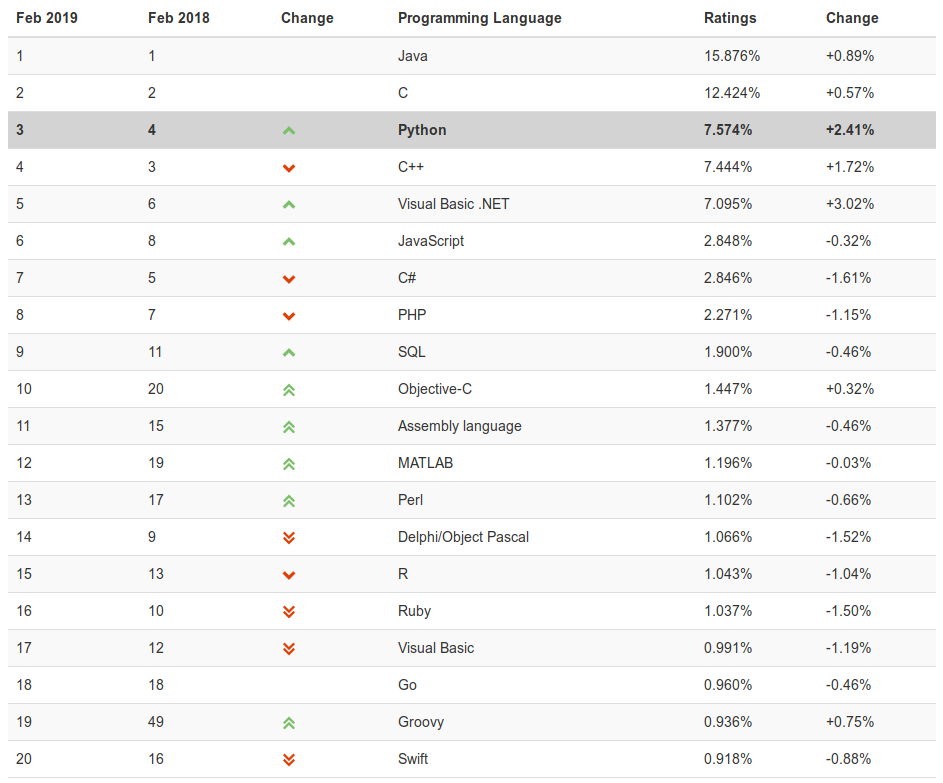
\includegraphics[width = 10cm]{img/TiobeIndex.png}
}



\frame{\frametitle{Python compared to other languages}
\rowcolors{1}{}{lightgray}
\begin{tabular}{c c c c c}
    & Python & C/C++ & Java & R 
\pause 
    \\ 
    Running speed & OK & Extremely fast & OK & Slow \pause \\  
    Easy to code? & Very easy & Extremely hard & Hard/OK & OK \pause \\  
    Portable? & Very easy & Hard & Very easy & Easy \pause \\  
    Documentation & Excellent & Very poor & Poor & Poor \pause \\  
\end{tabular}
}


\frame{\frametitle{Tables with pause}
\begin{tabular}{c c c}
A & B & C \\ 
\pause 
1 & 2 & 3 \\  
\pause 
A & B & C \\ 
\end{tabular} }

\frame{\frametitle{blocs}

\begin{block}{title of the bloc}
bloc text
\end{block}

\begin{exampleblock}{title of the bloc}
bloc text
\end{exampleblock}


\begin{alertblock}{title of the bloc}
bloc text
\end{alertblock}
}
\end{document}

